%% ---------------------------------------------------------------------------------------------------------
\section{Validity of the physical record}\label{sec:physics}

\paragraph{Question} The mechanism analysis uses logged contacts, distances and poses. Are these measurements trustworthy, and does any failure change a result?

\begin{table}[!htbp]
\centering\footnotesize
\caption{Measurement-validity checks on the development record (post hoc unless stated). S4--S6 were declared before the analysis; their official status is kept.}\label{tab:physics}
\input{\tabdir T5_physics_validity.tex}
\end{table}

\paragraph{Checks} We defined three checks before analysing the record (Table~\ref{tab:physics}). \emph{S4}: during a move, the minimum distance between robot geometry and the target cube stays positive. \emph{S5}: reconstructed penetrations between bodies do not exceed 1\,mm. \emph{S6}: for each contact pair listed by PhysX, the logged separation agrees with the gap we reconstruct from the logged poses and collision shapes within 1\,mm.

\paragraph{Evidence} S4 failed in one of 715 acted branches, an oracle branch ($-2.16$\,mm, policy seed 2, scene 51152), and in none of the V2 branches. S5 failed in two short events with fast-moving cubes (11 of 3,874 branch records: 400 trunks plus 9 arms in each of 386 triggered scene-runs). Replacing every logged collision mesh by its convex hull changed no S4 or S5 status (Fig.~\ref{fig:hull}). S6 \emph{failed}: 54,267 of 580,539 listed pair rows (9.3\%) disagreed by more than 1\,mm (Fig.~\ref{fig:s6}a).

\begin{figure}[!htbp]
\centering
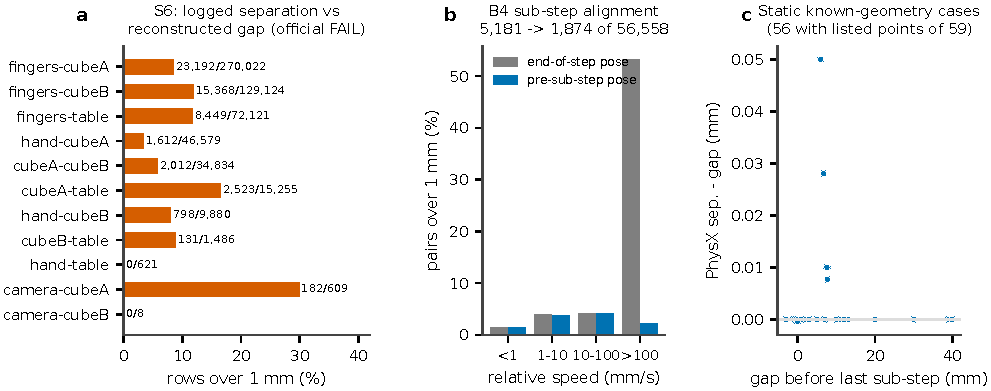
\includegraphics[width=\linewidth]{F7_physics_s6_b4.pdf}
\caption{Contact-separation check S6. (a) Rows over 1\,mm by pair kind (official FAIL). (b) Logging every physics sub-step on 11 used scene-runs: comparing with the pose before the last sub-step removes most disagreements of fast pairs. (c) Static boxes with known geometry: the PhysX separation equals the analytic gap before the last sub-step within 0.05\,mm.}\label{fig:s6}
\end{figure}

\paragraph{Partial explanation} Three follow-up measurements explain part of the S6 failure. First, on static box pairs with known geometry, the PhysX separation equals the analytic gap before the last sub-step within 0.05\,mm (Fig.~\ref{fig:s6}c), which fixes the definition of the logged quantity \cite{nvidia_physx_contact}. Second, logging every sub-step of 11 used scene-runs (re-run on the calibration host) showed that the contact list is computed at the pose before the last of the five sub-steps of a control step; comparing with that pose reduced the disagreements above 1\,mm from 5,181 to 1,874 of 56,558 pairs, and for pairs faster than 100\,mm/s from 3,436 to 146 (Fig.~\ref{fig:s6}b). Third, the remaining 1,874 rows are all zero-impulse proximity pairs between a finger box and a cube; shape-index mismatch and static edge geometry were excluded as causes. Their origin is not established.

\begin{figure}[!htbp]
\centering
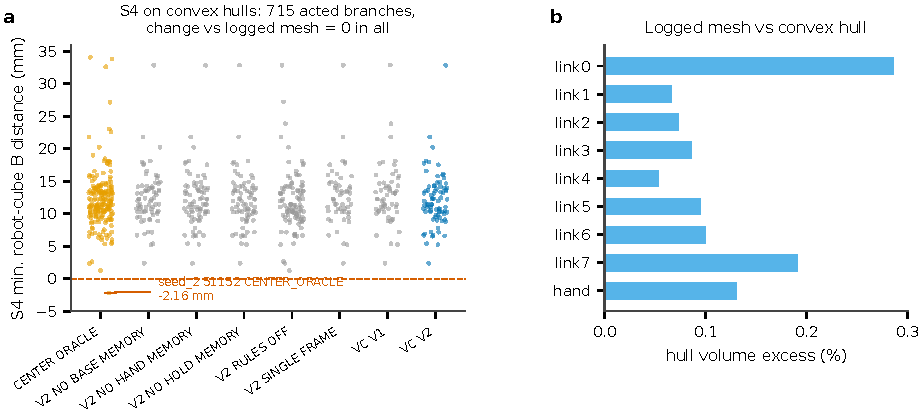
\includegraphics[width=\linewidth]{F8_hull_sensitivity.pdf}
\caption{Collision-geometry sensitivity. (a) S4 minimum robot--target distance on convex hulls for all 715 acted branches; the change with respect to the logged meshes is zero in every branch, and the only negative value is an oracle branch. (b) Volume excess of the convex hull over the logged mesh per link (at most 0.3\%).}\label{fig:hull}
\end{figure}

\paragraph{Interpretation} The task outcomes, the harm certificate and the efficacy test use only the success flag of each branch, which the simulator computes from its own state; they do not depend on S4--S6. The S6 failure limits the use of logged separations for fine-grained contact analysis, which is why we use them only descriptively.

\paragraph{Limits} S6 keeps its official FAIL status. No check here establishes continuous-time collision freedom; a contact between control steps can be missed.

